\chapter*{Data Model}
\section*{Overview}
\begin{center}
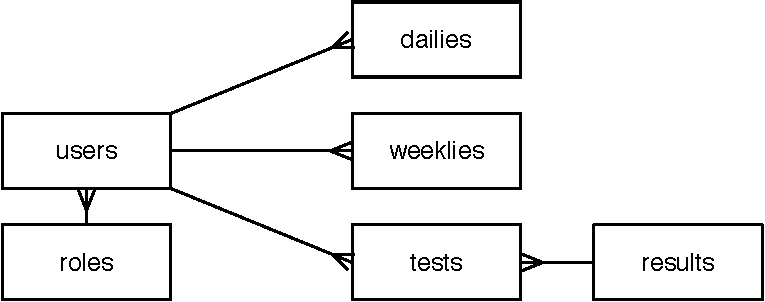
\includegraphics[width=0.8\textwidth]{./erd.pdf}
\end{center}
LOST concerns itself with three main ideas: assets, users, and security tags. \emph{Assets} are the entities that LOST has been designed to track. \emph{Users} represent OSNAP staff that are involved in managing assets. \emph{Security tags} are used to provide mandatory access control since there are limitations on which security compartments users are allowed to view or manage.

Several join tables appear in the model. These join tables are needed to handle the many-to-many relation ships between entities. 


\section*{Asset Tables}

\subsection*{products}
\begin{tabular}{l|l|l}
\hline
product\_pk & integer & primary key for a product instance \\
vendor & text & who sells this product \\
description & text & description of the asset \\
alt\_description & text & alternate description for the asset \\
\hline
\end{tabular}

\subsection*{assets}
\begin{tabular}{l|l|l}
\hline
asset\_pk & integer & primary key for an asset instance \\
product\_fk & integer & id for the product instance the asset was spawned from \\
asset\_tag & text & stick or engraved id used for inventory tracking \\
description & text & description of the asset \\
alt\_description & text & alternate description for the asset \\
\hline
\end{tabular}

\subsection*{vehicles}
\begin{tabular}{l|l|l}
\hline
vehicle\_pk & integer & primary key for an asset instance \\
asset\_fk & integer & id for the associated asset record \\
\hline
\end{tabular}

Vehicles are a type of asset but are special since they can be used to transport other assets. Table inheritance in Postgres could be used to do this a little more gracefully but that is an out of scope feature.

\subsection*{facilities}
\begin{tabular}{l|l|l}
\hline
facility\_pk & integer & primary key for a facility instance \\
fcode & text & facilities code used to identify the facility (6 or less characters) \\
common\_name & text & common name for the facility \\
location & text & addressing information for the facility \\
\hline
\end{tabular}

\subsection*{asset\_at}
\begin{tabular}{l|l|l}
\hline
asset\_fk & integer & asset at a facility \\
facility\_fk & integer & facility the asset is at \\
arrive\_dt & timestamp & when the asset arrived \\
depart\_dt & timestamp & when the asset left \\
\hline
\end{tabular}

\subsection*{convoys}
\begin{tabular}{l|l|l}
\hline
convoy\_pk & integer & primary key for a convoy instance \\
request & text & request identifier for the convoy \\
source\_fk & integer & source facility \\
dest\_fk & integer & destination facility \\
depart\_dt & timestamp & when the asset departed \\
arrive\_dt & timestamp & when the asset arrived \\
\hline
\end{tabular}

\subsection*{used\_by}
\begin{tabular}{l|l|l}
\hline
vehicle\_fk & integer & vehicle participating in a convoy \\
convoy\_fk & integer & convoy vehicle participates in \\
\hline
\end{tabular}

\subsection*{asset\_on}
\begin{tabular}{l|l|l}
\hline
asset\_fk & integer & asset at a facility \\
convoy\_fk & integer & convoy the asset is on \\
load\_dt & timestamp & when the asset was loaded \\
unload\_dt & timestamp & when the asset was unloaded \\
\hline
\end{tabular}


\section*{User Tables}

\subsection*{users}
\begin{tabular}{l|l|l}
\hline
user\_pk & integer & primary key for a user instance \\
username & text & login name used by the user \\
active & boolean & Is the user active? \\
\hline
\end{tabular}

\subsection*{roles}
\begin{tabular}{l|l|l}
\hline
role\_pk & integer & primary key for a role instance \\
title & text & short textual name for the role \\
\hline
\end{tabular}

\subsection*{user\_is}
\begin{tabular}{l|l|l}
\hline
user\_fk & integer & id for the user instance \\
role\_fk & integer & id for the role instance \\
\hline
\end{tabular}

\subsection*{user\_supports}
\begin{tabular}{l|l|l}
\hline
user\_fk & integer & id for the user instance \\
facility\_fk & integer & id for the facility instance \\
\hline
\end{tabular}


\section*{Security Tables}

\subsection*{levels}
\begin{tabular}{l|l|l}
\hline
level\_pk & integer & primary key for security level lookups \\
abbrv & text & abbreviation for the security level \\
comment & text & comment, if any \\
\hline
\end{tabular}

\subsection*{compartments}
\begin{tabular}{l|l|l}
\hline
compartment\_pk & integer & primary key for compartment lookups \\
abbrv & text & abbreviation for the security compartment \\
comment & text & comment, if any \\
\hline
\end{tabular}

\subsection*{security\_tags}
\begin{tabular}{l|l|l}
\hline
tag\_pk & integer & primary key for security tag instance \\
level\_fk & integer & id for the tag level \\
compartment\_fk & integer & id for the tag compartment \\
user\_fk & integer & user the tag is applied to or NULL \\
product\_fk & integer & product the tag is applied to or NULL \\
asset\_fk & integer & asset the tag is applied to or NULL \\
\hline
\end{tabular}

Security tags must have both level and compartment. Security tags must also have a user xor product xor asset.

